\section{Shared Instruction Cache Design}
%\jbs{Akhil in charge.}

%% \begin{figure}[ht!]
%% \centering
%% 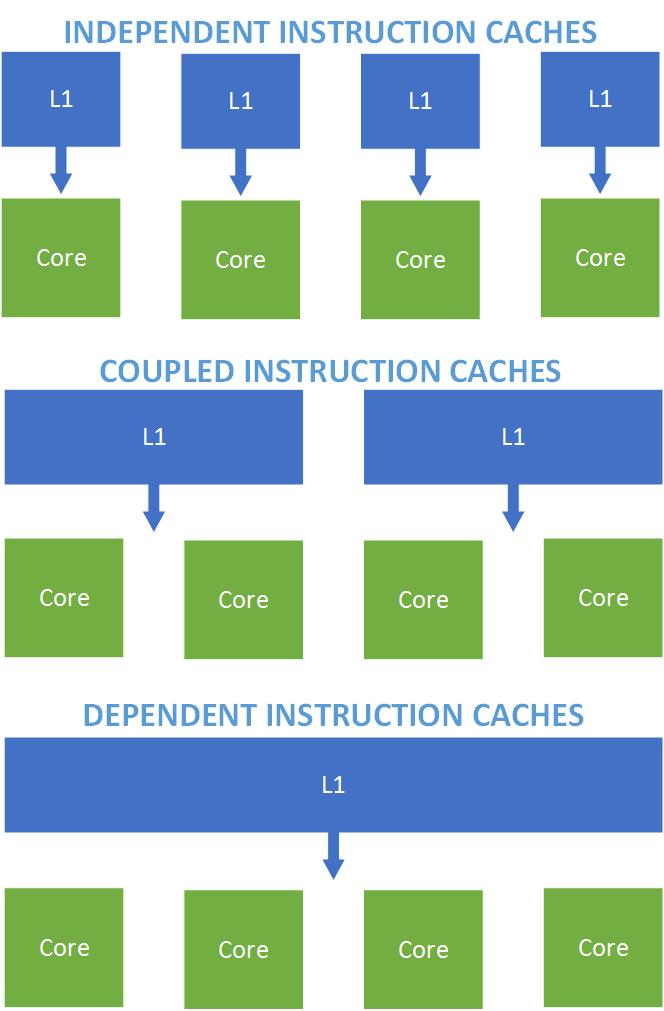
\includegraphics[width=90mm]{graphics/InstructionCacheDesignSketches.jpg}
%% \caption{(a) Current design of Instruction Caches in an SM, (b) Proposed cache design 1 (b) Proposed cache desgn 2.}
%% \label{propDesign}
%% \end{figure}

\begin{figure}[ht!]
\centering
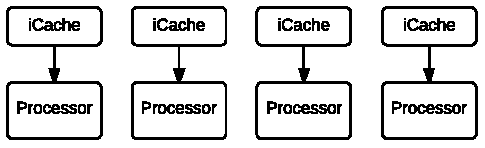
\includegraphics[width=\columnwidth]{graphics/IndependentCaches}
\caption{Independent instruction caches}
\label{fig:indep}
\end{figure}

Most computer architectures build an independent instruction cache for
each processing core as seen in Figure~\ref{fig:indep}.
Reducing the number of instruction caches for the same number of cores
in a multi-core processor may have certain advantages. 
First, a shared instruction cache design could reduce the amount of
storage and die area required to hold instructions on chip when
multiple processors are executing the same program.
This advantage in storage and area could result in reduced performance
if the pressure to this shared resource becomes too high.
Similarly, the benefits of reduced cache size will not be realized in
multi-program workloads, unless the operating system is able to
discover shared library code and perform the proper virtual mapping to
allow the hardware to exploit it.
Second, a shared instruction cache design could reduce the number of
compulsory misses because an instruction previously fetched
by one processor may be available for another processor immediately
rather than requiring an additional cache miss. 
Again, this benefit is only relevant for single-application parallel
workloads. 

\begin{figure}[ht!]
\centering
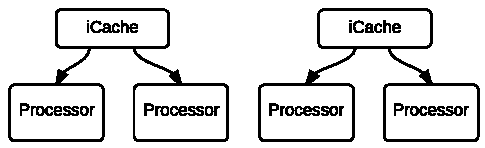
\includegraphics[width=\columnwidth]{graphics/PairedCaches}
\caption{Partly shared instruction caches}
\label{fig:paired}
\end{figure}

The first approach to shared instruction caches would be to couple an
instruction cache with a pair of processors as in
Figure~\ref{fig:paired}. 
This would have a small amount of routing overhead and allow for the
operating system to intelligently schedule two threads that share
instructions to these two processor cores in order to exploit this
sharing. 
However, if an application wanted more sharing, the benefits beyond
only two cores would be smaller.
As a limit, a chip could be designed to share a single instruction
cache among all processors on chip, shown with an example of only four
processors in Figure~\ref{fig:shared}.
For an arbitrary number of cores, this level of sharing could be
scaled up or down to fit the applications and purpose of the
architecture design.
One could even imagine a design where assymetrical sharing is enabled
by grouping different sets of compute cores differently and then
assigning the application threads to the appropriate cores to match
the sharing to the hardware available.

\begin{figure}[ht!]
\centering
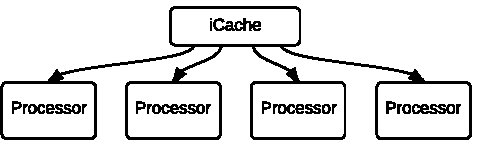
\includegraphics[width=\columnwidth]{graphics/SharedCaches}
\caption{Fully shared instruction caches}
\label{fig:shared}
\end{figure}

While our proposed technique is likely only beneficial in situations
with highly parallel programs, it is likely that future systems will
often run a few highly parallel workloads that can benefit from these
advantages. 

\jbs{Consider adding text about banked cache designs and how that
  would increase parallel cache performance.}
 




